\section{Evaluation}

\subsection{Measuring bias of spectrometer}
To be able to identify the absorption spectrum of the iodine 2 molecule, we have to analise 
the measurements for callibration with the Na- and Hg-vapour lamps, respectively. The measured
spectrum over the entire range of the spectrometer is plotted in figure \ref{fig:specturm_all}. 
To locate the maxima, we magnify the recordings in a region around the corrispoding maximum. 
For sodium, this is done in figure \ref{fig:na_max}. One can see the two characteristic peaks 
at 
\begin{eqnarray*}
    \lambda_\mathrm{max, 1} = 589.1 \pm \unc \nm \\
    \lambda_\mathrm{max, 2} = 589.6 \pm \unc \nm.
\end{eqnarray*}
The uncertainty of \unc is taken from the value given in \cite{}, being half the value of 
resolution (6nm). It corrisponds with the sharpness of the maxima 
(fwhm about 0.4nm as seen in the figures). 
These corrispond with the values given in literature \cite{}, namely 
\begin{eqnarray*}
    \lambda_\mathrm{max, 1} = 589.0 \nm \\
    \lambda_\mathrm{max, 2} = 589.6 \nm.
\end{eqnarray*}
In the recorded spectrum, we also see another, smaller peak at 
\begin{equation}
    \lambda = 588.4 \pm \unc \nm.
\end{equation} 
This peak is not found in literature \cite{nist} and seems to be an artefact of the measurement. 
In fact, as the light from the Na lamp was not colliminated and focused very well, one could 
suspect diffration at the entrance of the spectrometer as the cause, as the spectrometer 
doesn't measure wavelength directly but rather the intensity corrisponding to a certain angle. 

For the Hg lamp, we observe similar results. As seen in \ref{fig:spectrum_all}, intensities 
of the minima varied quiet drastically. For that reason, we took various measurements of which 
we can use one for the first maximum (fig. \ref{fig:hg1_max}) and another at much lower 
intensity for the three other ones (figs. \ref{fig:hg2_max}, \ref{fig:hg3_max}). 
We identify the following maxima:
\begin{eqnarray*}
    \lambda_\mathrm{max, 1} &=& 435.5 \pm \unc \ (435.83)\nm \\
    \lambda_\mathrm{max, 2} &=& 545.9 \pm \unc \ (545.9)\nm \\
    \lambda_\mathrm{max, 3} &=& 576.8 \pm \unc \ (576.8)\nm \\
    \lambda_\mathrm{max, 4} &=& 576.9 \pm \unc \ (576.9)\nm.
\end{eqnarray*}
The values in parenthesis cite literature values \cite{}. \\
As the spectrometer yields results lying within the literature values for the 
stated uncertainty, we conclude that there is no bias in the measured wavelength.

\begin{figure}
\centering
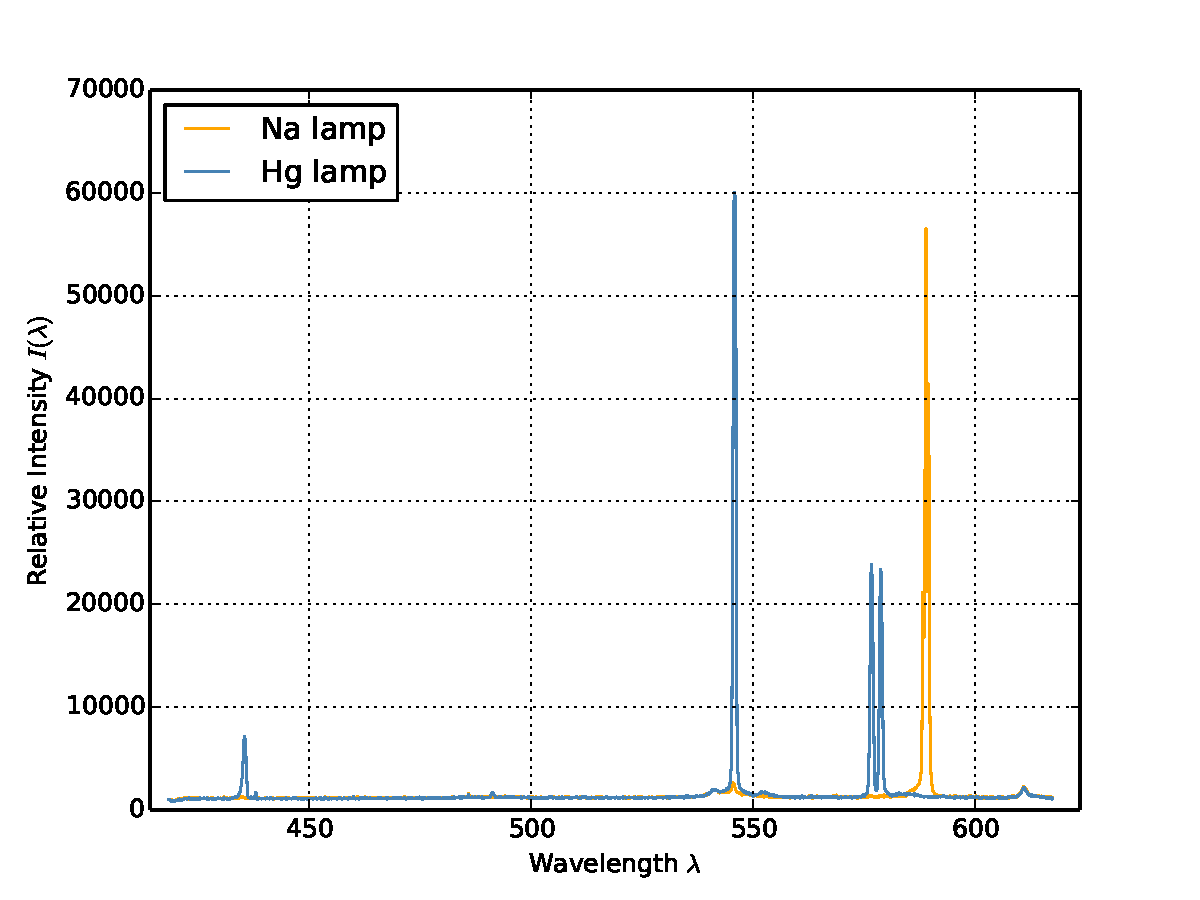
\includegraphics[width=\pltw]{analysis/figures/spectrum_all.pdf}
\caption{Measured spectrum of Na and Hg lamp}
\label{fig:spectrum_all}
\end{figure}

\begin{figure}
\centering
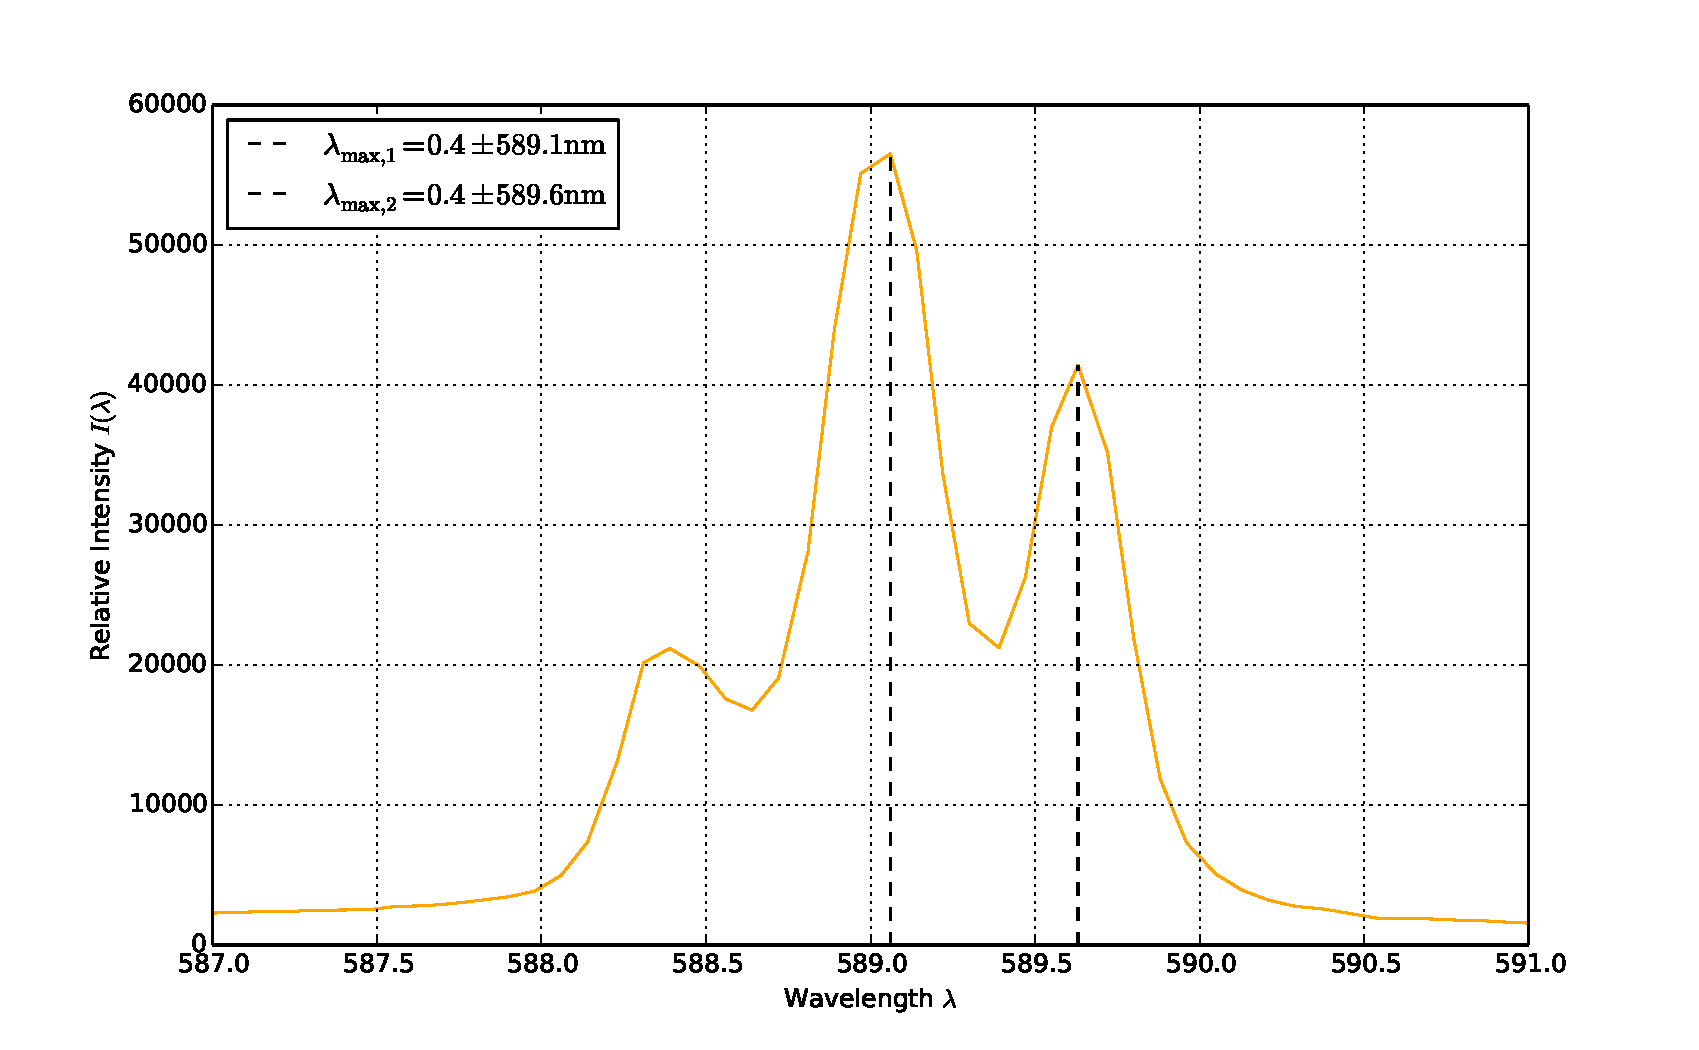
\includegraphics[width=\pltw]{analysis/figures/na_max.pdf}
\caption{Measured spectrum of the Na lamp, detail at the 
characteristic orange double line}
\label{fig:na_max}
\end{figure}

\begin{figure}
\centering
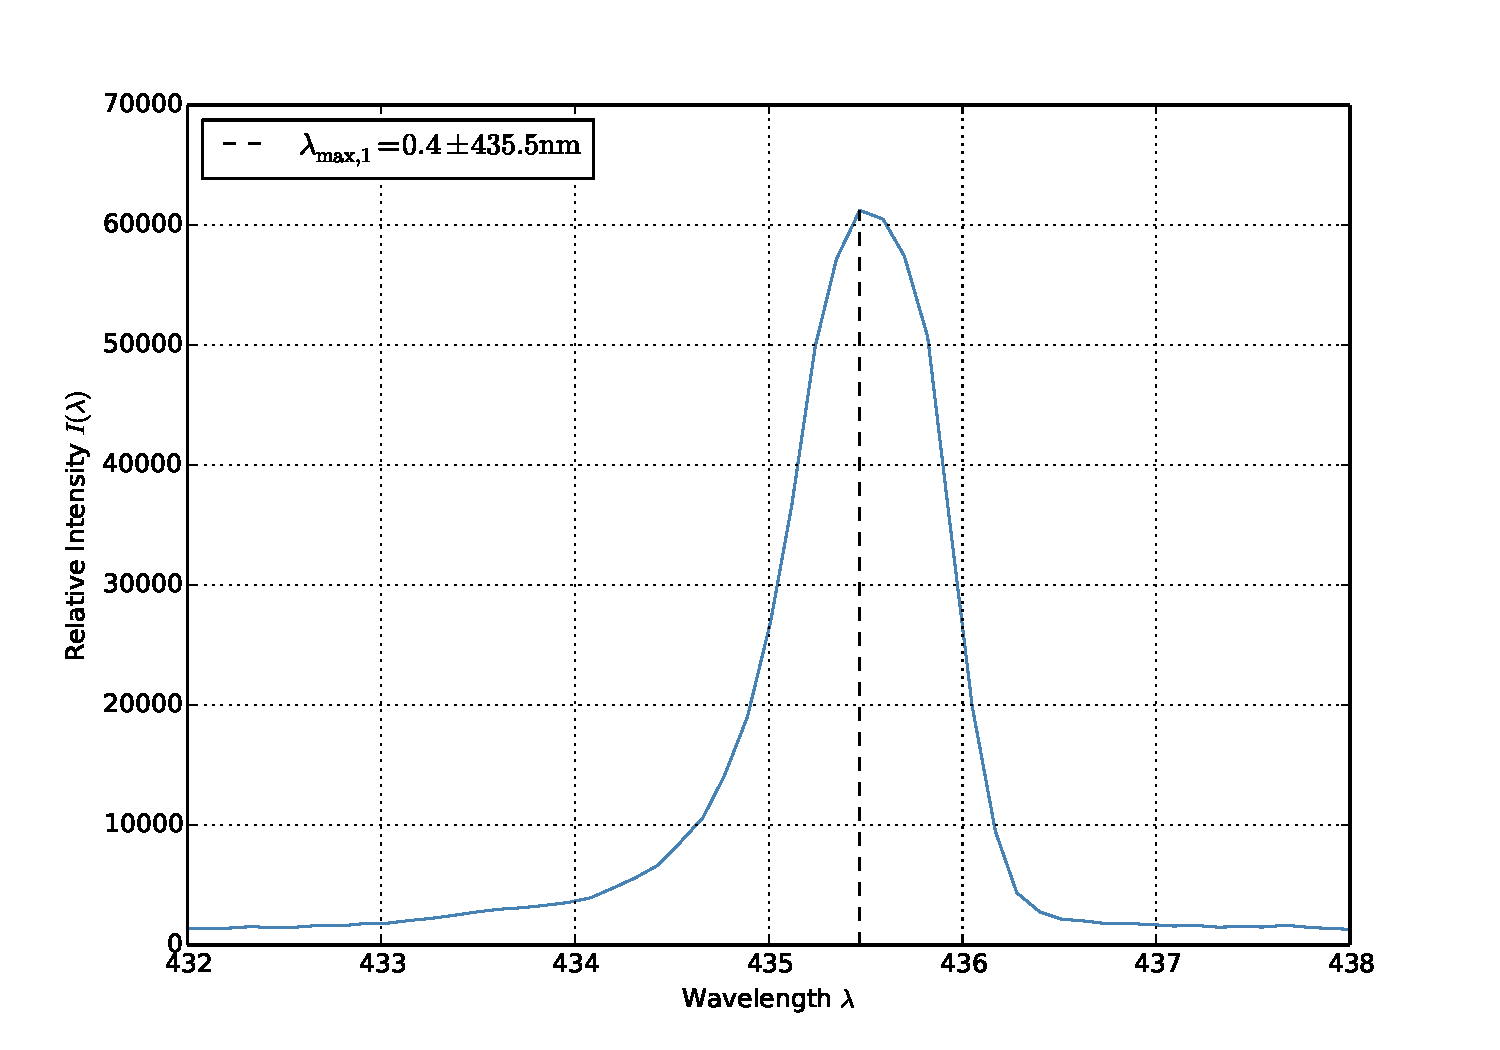
\includegraphics[width=\pltw]{analysis/figures/hg1_max.pdf}
\caption{Measured spectrum of the hg lamp, detail at first maximum}
\label{fig:hg1_max}
\end{figure}

\begin{figure}
\centering
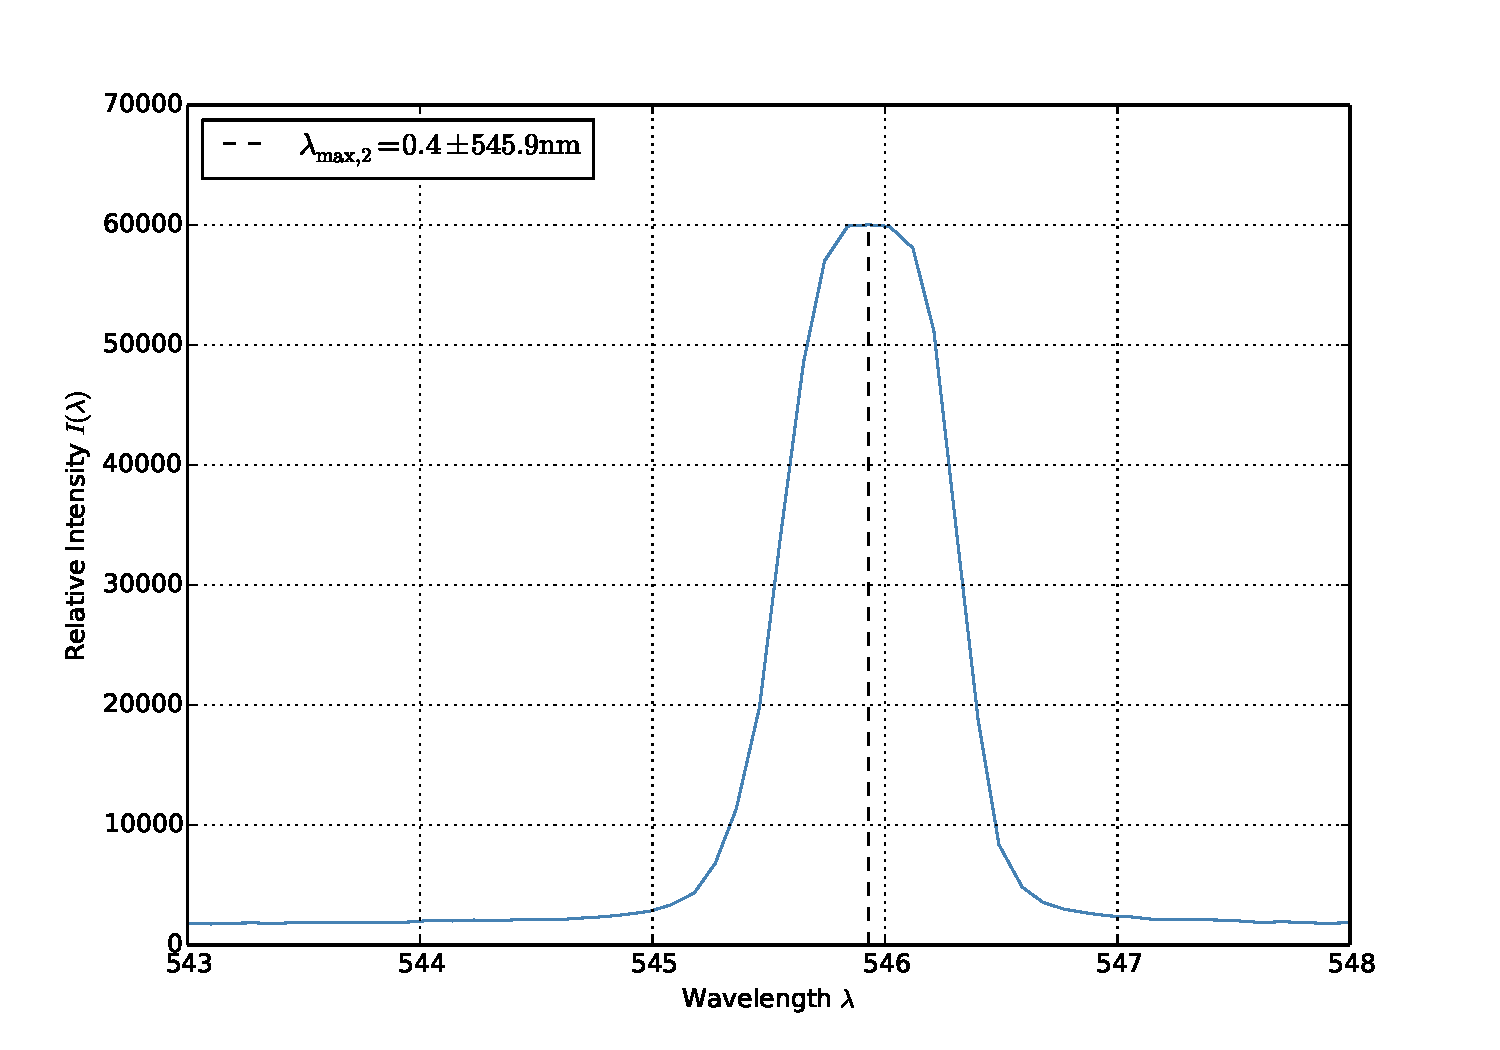
\includegraphics[width=\pltw]{analysis/figures/hg2_max.pdf}
\caption{Measured spectrum of the hg lamp, detail at second maximum}
\label{fig:hg2_max}
\end{figure}

\begin{figure}
\centering
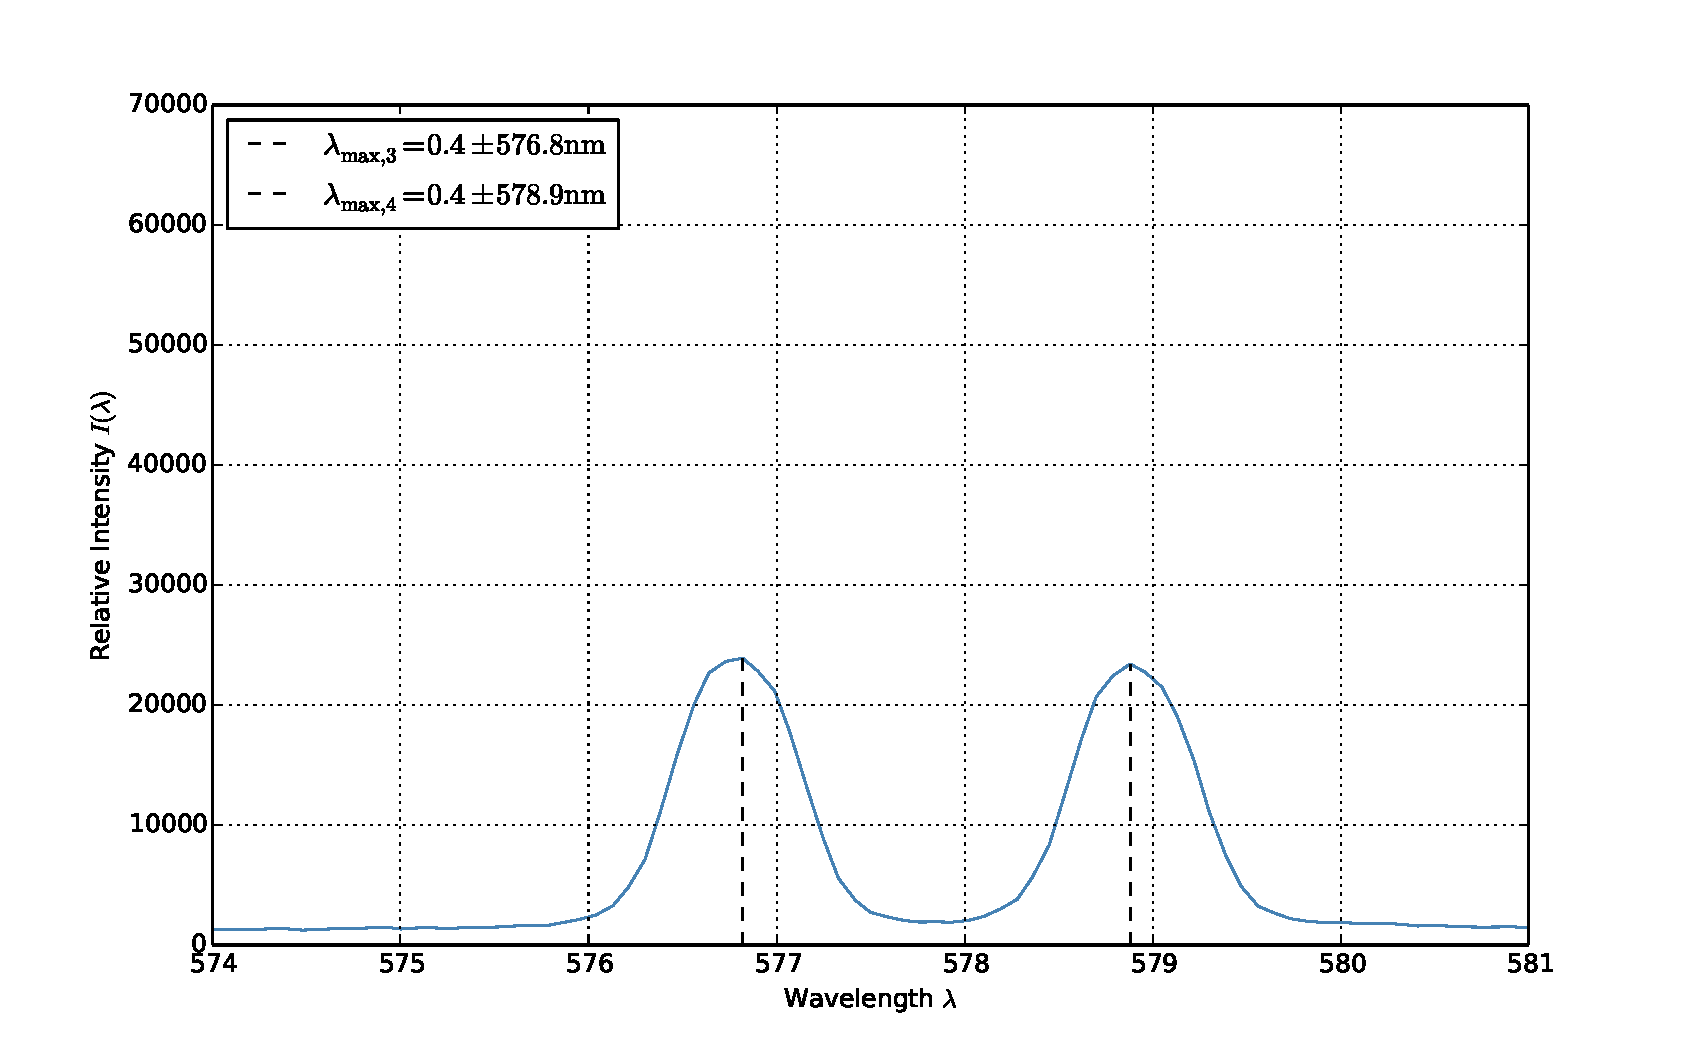
\includegraphics[width=\pltw]{analysis/figures/hg3_max.pdf}
\caption{Measured spectrum of the hg lamp, detail at thrid and fourth maximum}
\label{fig:hg3_max}
\end{figure}

\subsection{Spectrum of halogen lamp}
As we look out to measure the absorption spectrum of iodine, we first take a quick look at 
the specturm of the background from which photons are to be absorbed. The measured spectrum 
of the used halogen lamp within the range of wavelength in question is shown in figure 
\ref{fig:specturm_halogen_full}.
\begin{figure}
\centering
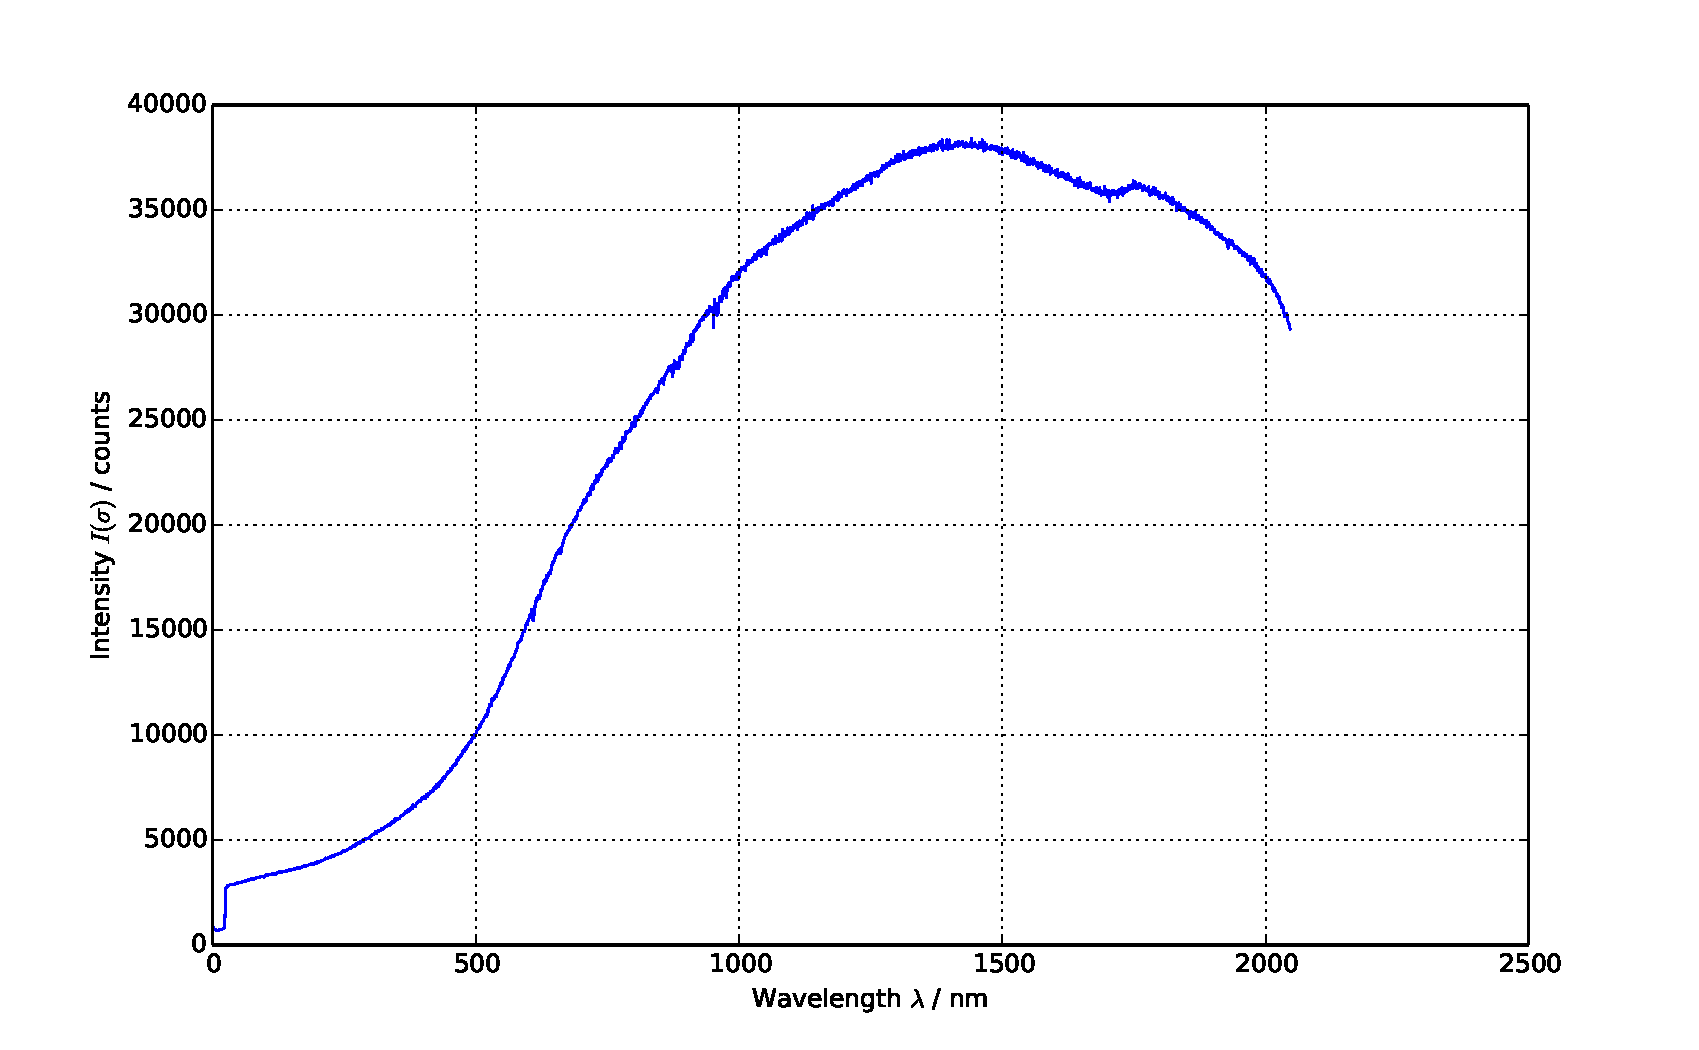
\includegraphics[width=\pltw]{analysis/figures/halogen_02.pdf}
\caption{Measured spectrum of the halogen lamp over the entire spectrum, no coerrection for 
diffraction in light}
\label{fig:spectrum_halogen_full}
\end{figure}
To be able to compare this to the absorption spectrum, we firth need to make the same 
corrections for diffraction in light as we do for the latter. We do so by linearly 
interpolating given literature values of the diffraction index, given in table 
\ref{tab:diff_air}.

\begin{table}[h]
\centering
\begin{tabular}{| c |l|l|l|l|}
\hline
$\lambda [\nm]$              & 680  & 600  & 540  & 500 \\ \hline
$(n_\mathrm{air} - 1) \cdot 10^{-4}$ & 2.76 & 2.77 & 2.78 & 279 \\ \hline
\end{tabular}
\caption{Diffraction indices for air at room temperatur and normal pressure for 
chosen wavelength $\lambda$, taken from \cite{}.}
\label{tab:diff_air}
\end{table}

The linear interpolation is done by the following equation:
\begin{eqnarray}
    n_\lambda &=& \frac{(2.79 - 0.01 j)}{10 ^{4}} - \
    \frac{(\lambda - \lambda_\mathrm{lower})} {10^{6} \cdot \
(\lambda_\mathrm{upper} - \lambda_\mathrm{lower})} + 1 \\
    \lambda &=& n_\lambda \, \lambda,
    \label{eqn:lin_interpol}
\end{eqnarray}
where j is the index of the collum of table \ref{tab:diff_air} within which $\lambda$ lies, 
$\lambda_\mathrm{upper}$ and $\lambda_\mathrm{lower}$ are the upper and lower bounds of the 
intervall (more precisely: $\lambda \in (\lambda_\mathrm{upper}, \lambda_\mathrm{lower}]$ ). 

The corrected values of $\lambda$ are now restricted to values of 
$\lambda \in [500\nm, 620\nm]$ and converted to $\cm$ by taking th inverse. The result 
can be observed in figure \ref{"fig:spectrum_halogen_red"}.
\begin{figure}
\centering
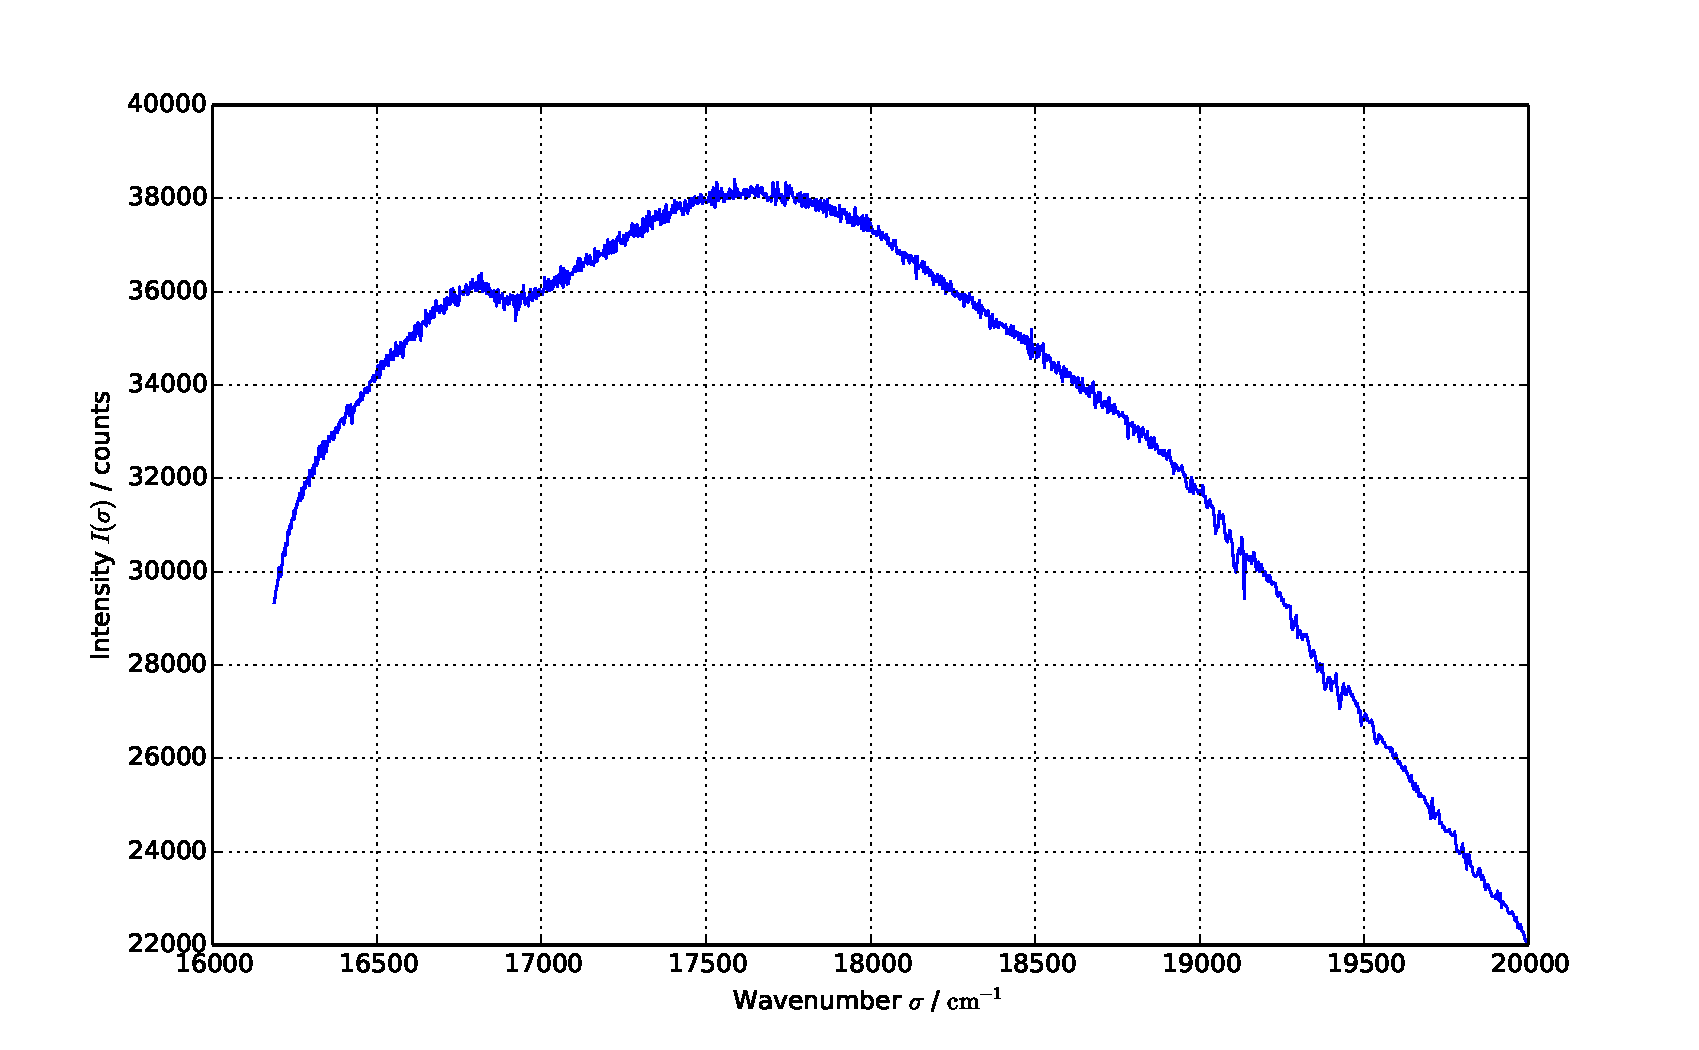
\includegraphics[width=\pltw]{analysis/figures/halogen_red.pdf}
\caption{Measured spectrum of the halogen lamp over reduced range, corrected for diffraction}
\label{fig:spectrum_halogen_red}
\end{figure}

\FloatBarrier

\subsection{Iodine absorption spectrum}

\subsubsection{Identifying progressions}
The process of identifying progressions turned out to be quiet difficult – reflecting the 
rather unsteady course of history. 
The absorption spectrum and the found progressions are shown in figure \ref{fig:absorp}.
The measured wavelenghts are reduced to vacuum wavelength by equation \eqref{eqn:lin_interpol} 
and then transformed to wavenumbers in $\cm$. 
As a first step, we preselected minima by an algorithm checking for each point to be lower than 
its four neighbouring points and added further points by hand later on. For identifying corrisponding 
progression to each of the selected points, we used the starting point of the 'zeroth progression' 
$v'' = 0  \rightarrow v' = 25$ with a band at $545.8 \nm = 18321 \cm$, as given by \cite{}. In our 
measurement, we found a mimima at $\sigma_{0, 25} = 18319 \pm 10\nm$. From that line, we could first 
identify the progression members down to $v' = 47$, where the last three points could be added using 
the first order approximation of the energy differences, namely their negative linear correlation 
to the energy (see figure \ref{fig:absorp_detail_03}). We then used the same relationship to identify 
points for $v' < 25$, which overlap with point of the progression $v''(1) \rightarrow v'$, the 
'first progression', 
as shown in figure \ref{fig:absorp_detail_02}. For this progression, we found much less values, as 
it overlaps with the progression $v''(1) \rightarrow v'$, 'second progression', as well, as one can 
observe in figure \ref{fig:absorp_detail_01}. All identified points with respective wavenumbers 
$\sigma_{v'', v'}, v'' \in \{0, 1, 2\}$ are shown in table \ref{tab:prog}, 
while the energy differences $\Delta G_{v''}(v' + 1 / 2) = \sigma_{v'', v'} - \sigma_{v'', v' + 1}$ are 
listed in table \ref{tab:dG}.

\begin{table}[h]
\centering
\small
\input{"analysis/table1.txt"}
\caption{Identified members of progressions of vibrational modes $v'' \rightarrow v'$ 
and corrisponding wavenumbers $\sigma_{v'', v'} = G'(v') - G''(v'')$ with uncertainties
$\Delta \sigma_{0, v'}$. }
\label{tab:prog}
\end{table}

\begin{table}[h]
\centering
\small
\input{"analysis/table2.txt"}
\caption{Differences in energy 
$\Delta G_{v''} = \Delta G_{v''} (v' + \frac{1}{2}) = G_{v''}(v') - G_{v''}(v' + 1)$ 
between successive members of the progressions $v'' \rightarrow v'$, $v'' \in \{0, 1, 2\}$. 
$ \Delta (\Delta G) $ are the corresponding uncertainties. 
 }
\label{tab:dG}
\end{table}

\begin{figure}
    \centering
    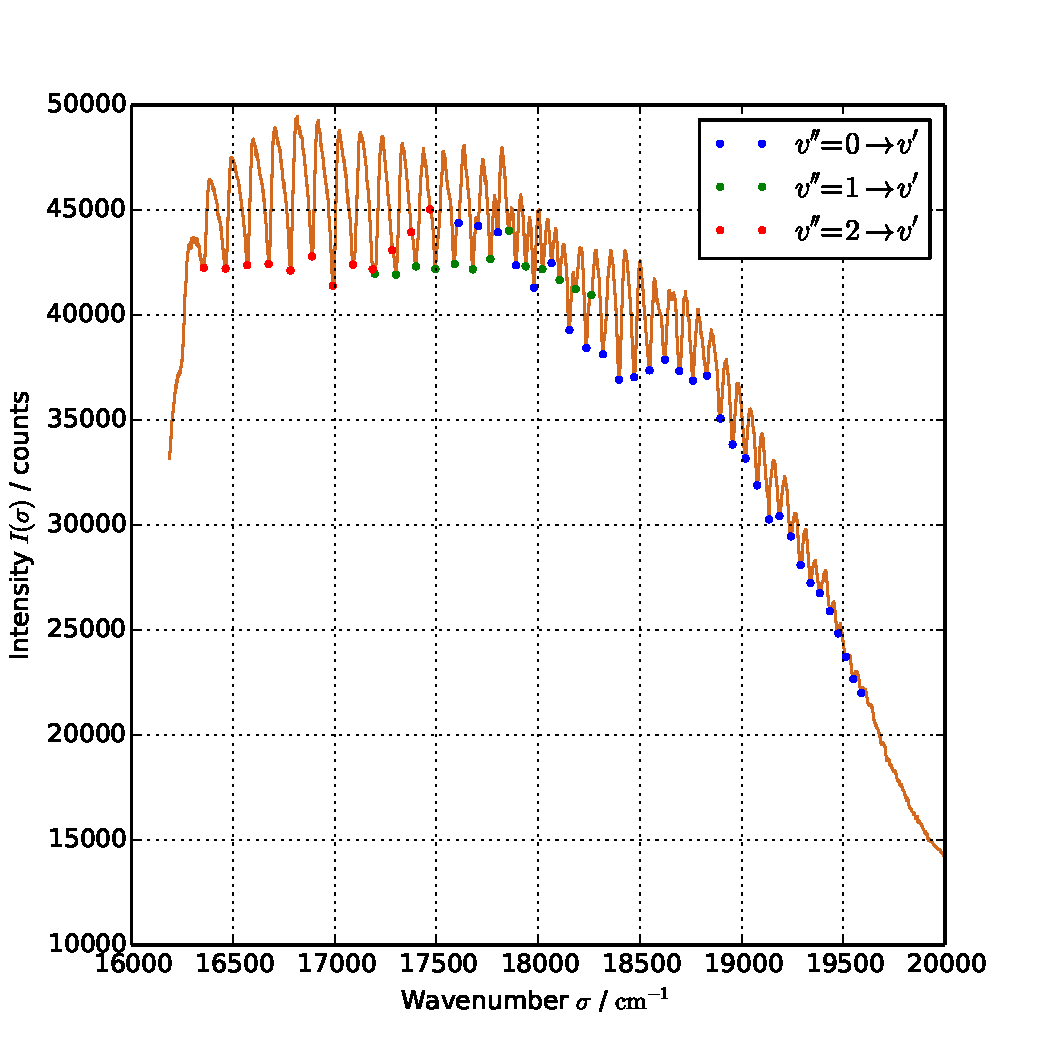
\includegraphics[width=\pltw]{analysis/figures/absorp_03.pdf}
    \caption{Measured absorption spectrum of iodine 2 molecules. The plot show the spectrum of 
    the halogen lamp having passed the iodine pipe. The local minima correspond to maxima of 
    absorption of the iodine. Three progressions of vibrational states $v'' \rightarrow v'$
    within the electronic transition 
    $B ^3\Pi_{\sigma \, \mathrm{u}}^{+} \quad \leftarrow \quad X ^1\Sigma_{\sigma \, \mathrm{u}}^{+}$ 
    are identified with colored dots. }
    \label{fig:absorp}
\end{figure}

\begin{figure}
    \centering
    \begin{subfigure}[b]{\mpltw}
        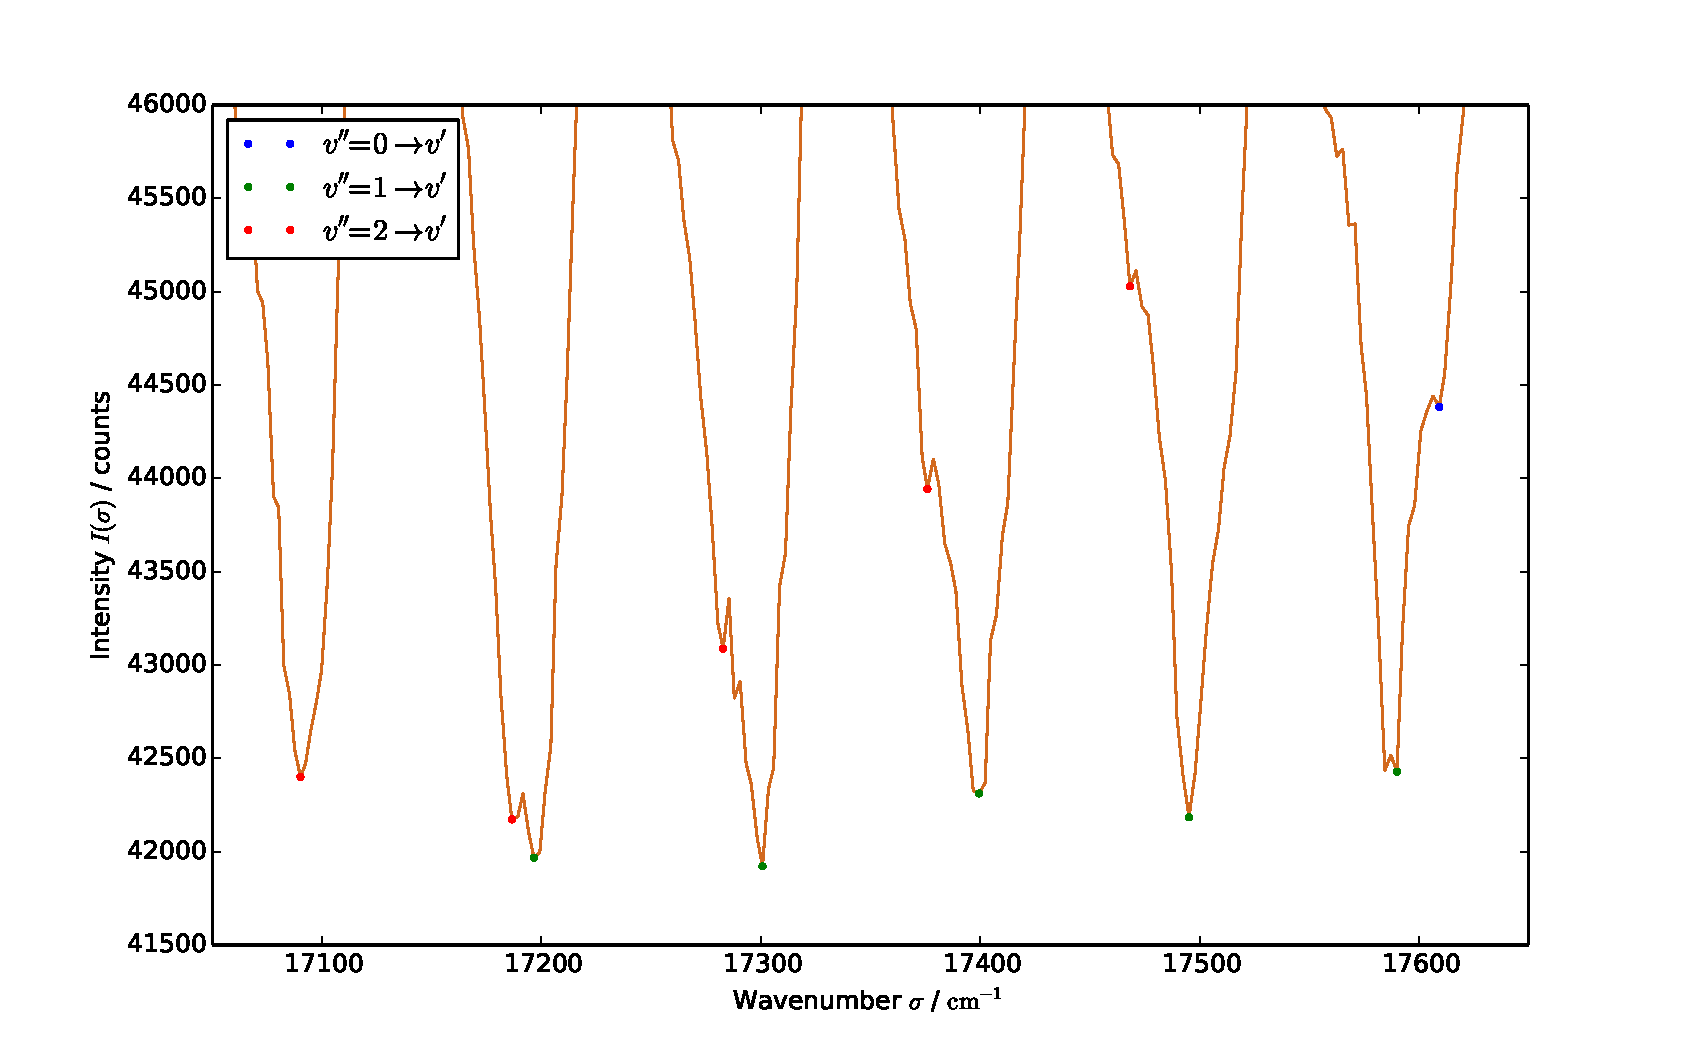
\includegraphics[width=\textwidth]{analysis/figures/absorp_03_detail_01.pdf}
        \caption{Overlap of $v'=1$ and $v'=2$}
        \label{fig:absorp_detail_01}
    \end{subfigure}\qquad
    \begin{subfigure}[b]{\mpltw}
        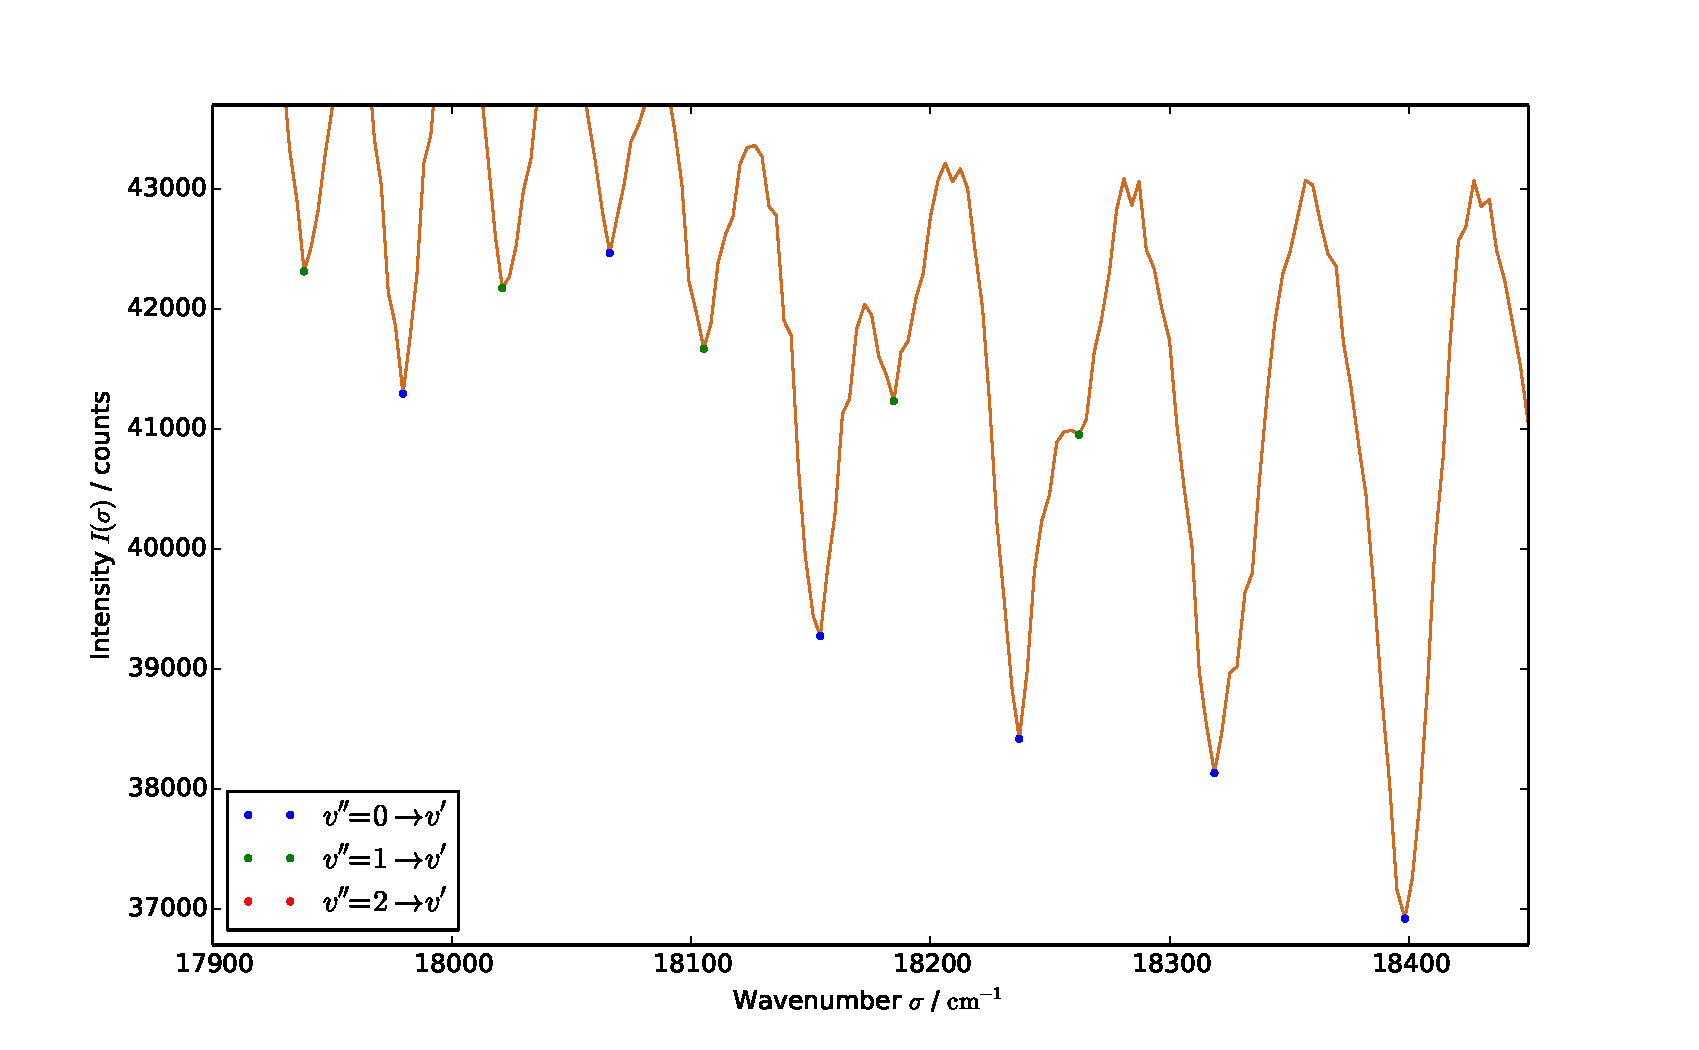
\includegraphics[width=\textwidth]{analysis/figures/absorp_03_detail_02.pdf}
        \caption{Overlap of $v'=0$ and $v'=1$"}
        \label{fig:absorp_detail_02}
    \end{subfigure}
    \begin{subfigure}[b]{\mpltw}
        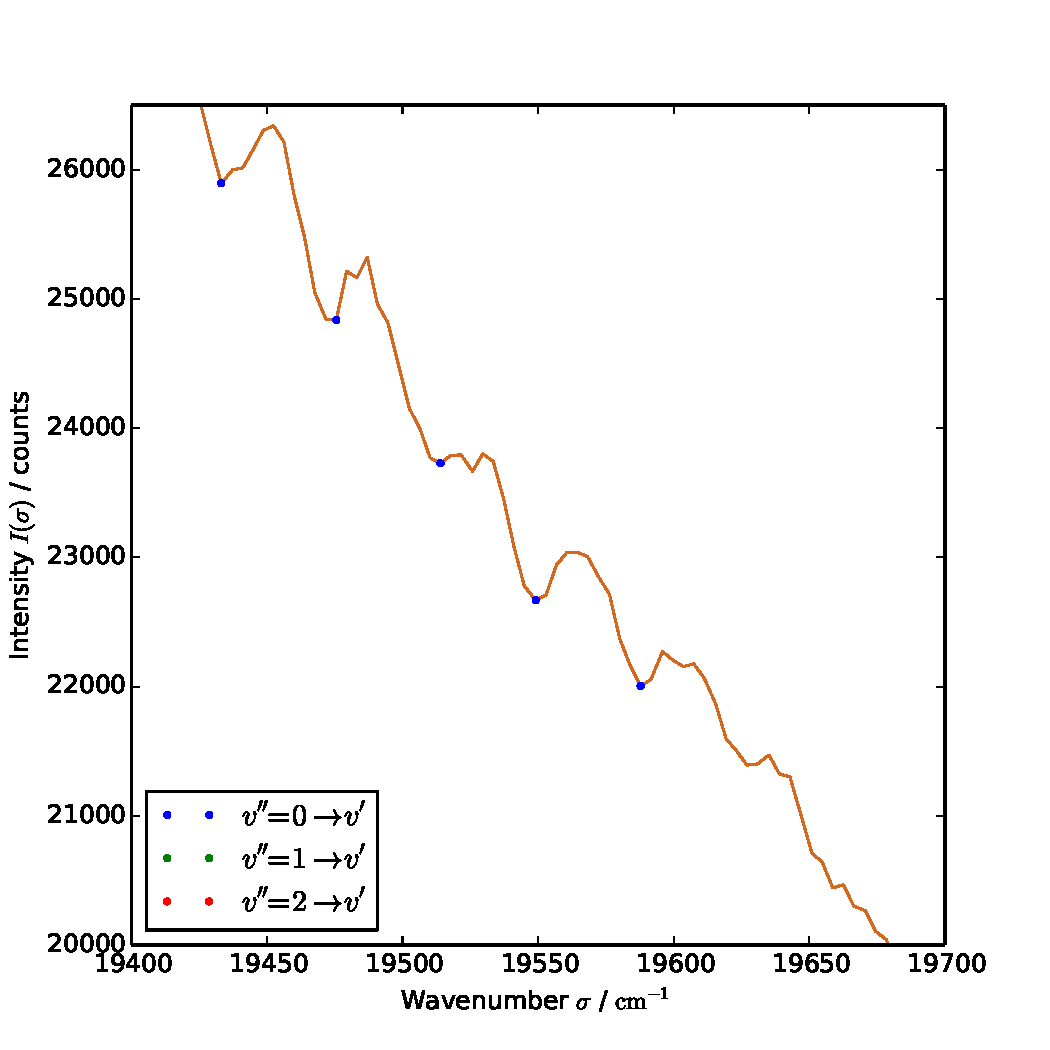
\includegraphics[width=\textwidth]{analysis/figures/absorp_03_detail_03.pdf}
        \caption{End of $v'=0'$}
        \label{fig:absorp_detail_03}
    \end{subfigure}
    \caption{Details of \ref{fig:absorp}: members of progressions at points, where 
    identification is done manually, comparing with \cite{staatsexamen}.
    }
    \label{fig:absorp_detail}
\end{figure}



\FloatBarrier

\subsubsection{Birge-Sponer plots}
The energy differences $\Delta G_{v''}(v' + 1/2)$ of the identified progressions can 
be plotted over the corresponding wavenumbers $v' + 1/2$. The resulting so-called 
Birge-Sponer plots, figures 
\ref{fig:b_s_0},  \ref{fig:b_s_1},  \ref{fig:b_s_2}, 
are used to calculate the vibrational constants $\omega_e'$ and $\omega_e' x_e'$. 

% Birge Sponer plots
\begin{figure}
    \centering
    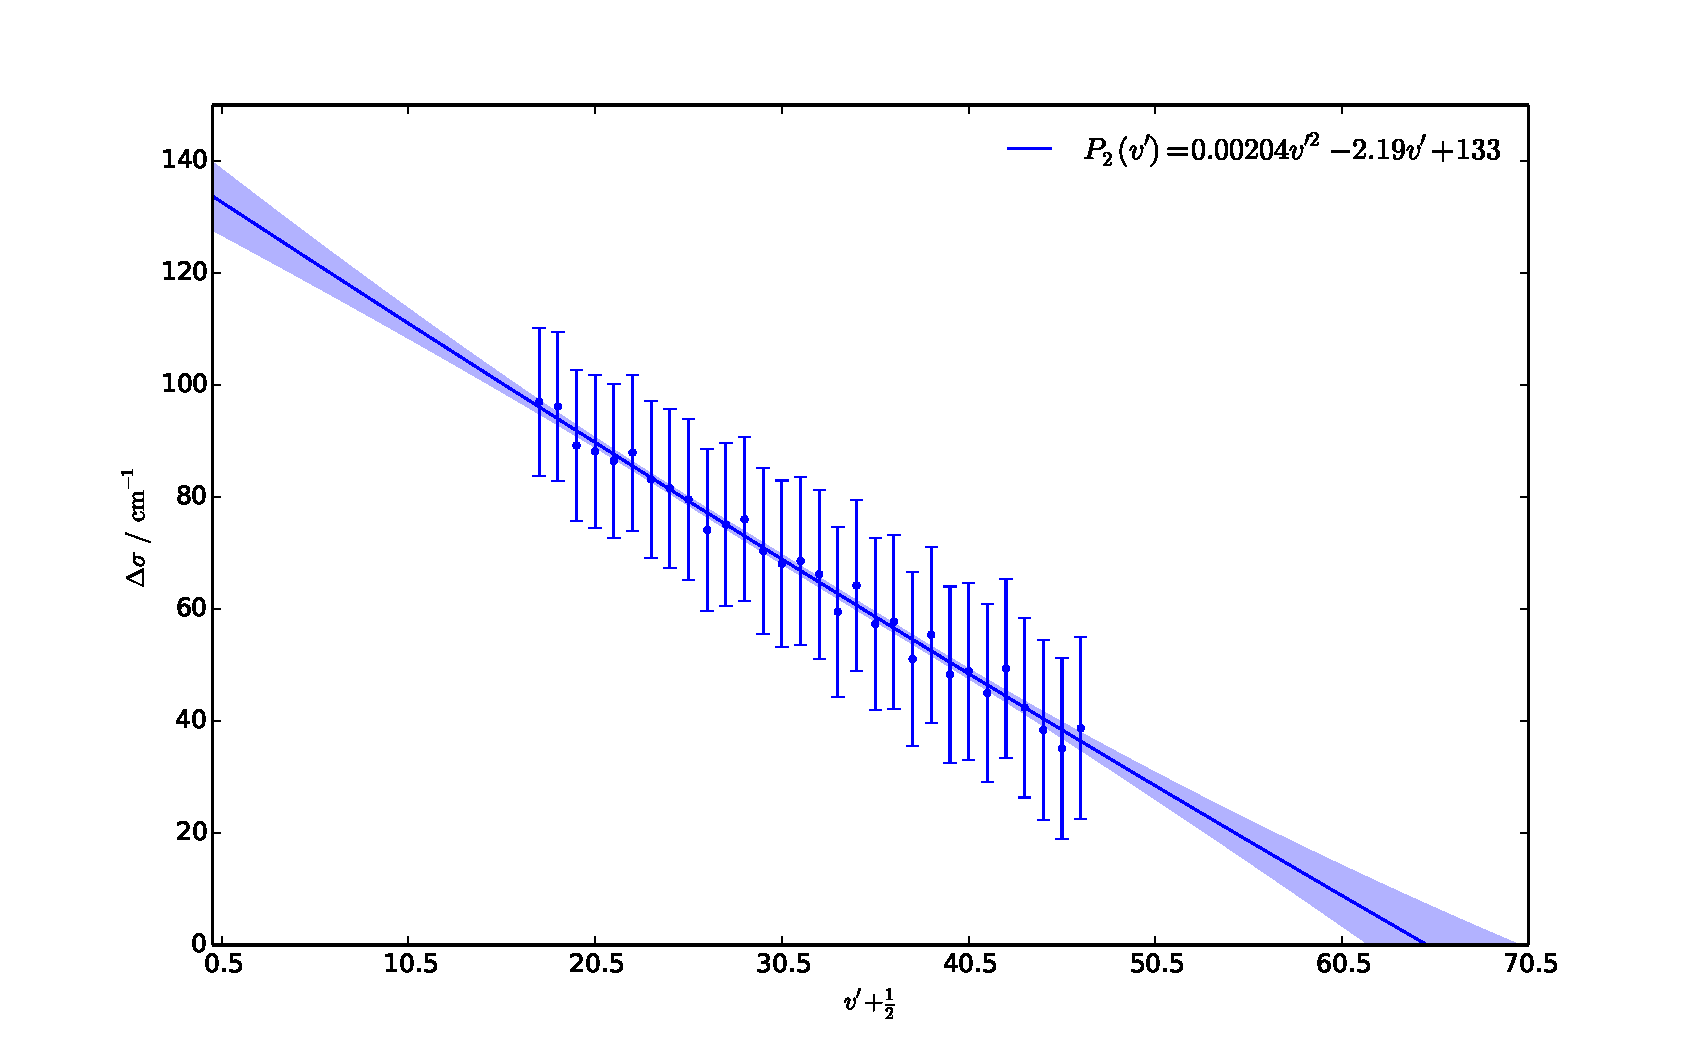
\includegraphics[width=\pltw]{analysis/figures/b_s_0.pdf}
    \caption{Birge-Sponer plot for the progression $v'' = 0 \rightarrow v'$.  
    }
    \label{fig:b_s_0}
\end{figure}

\begin{figure}
    \centering
    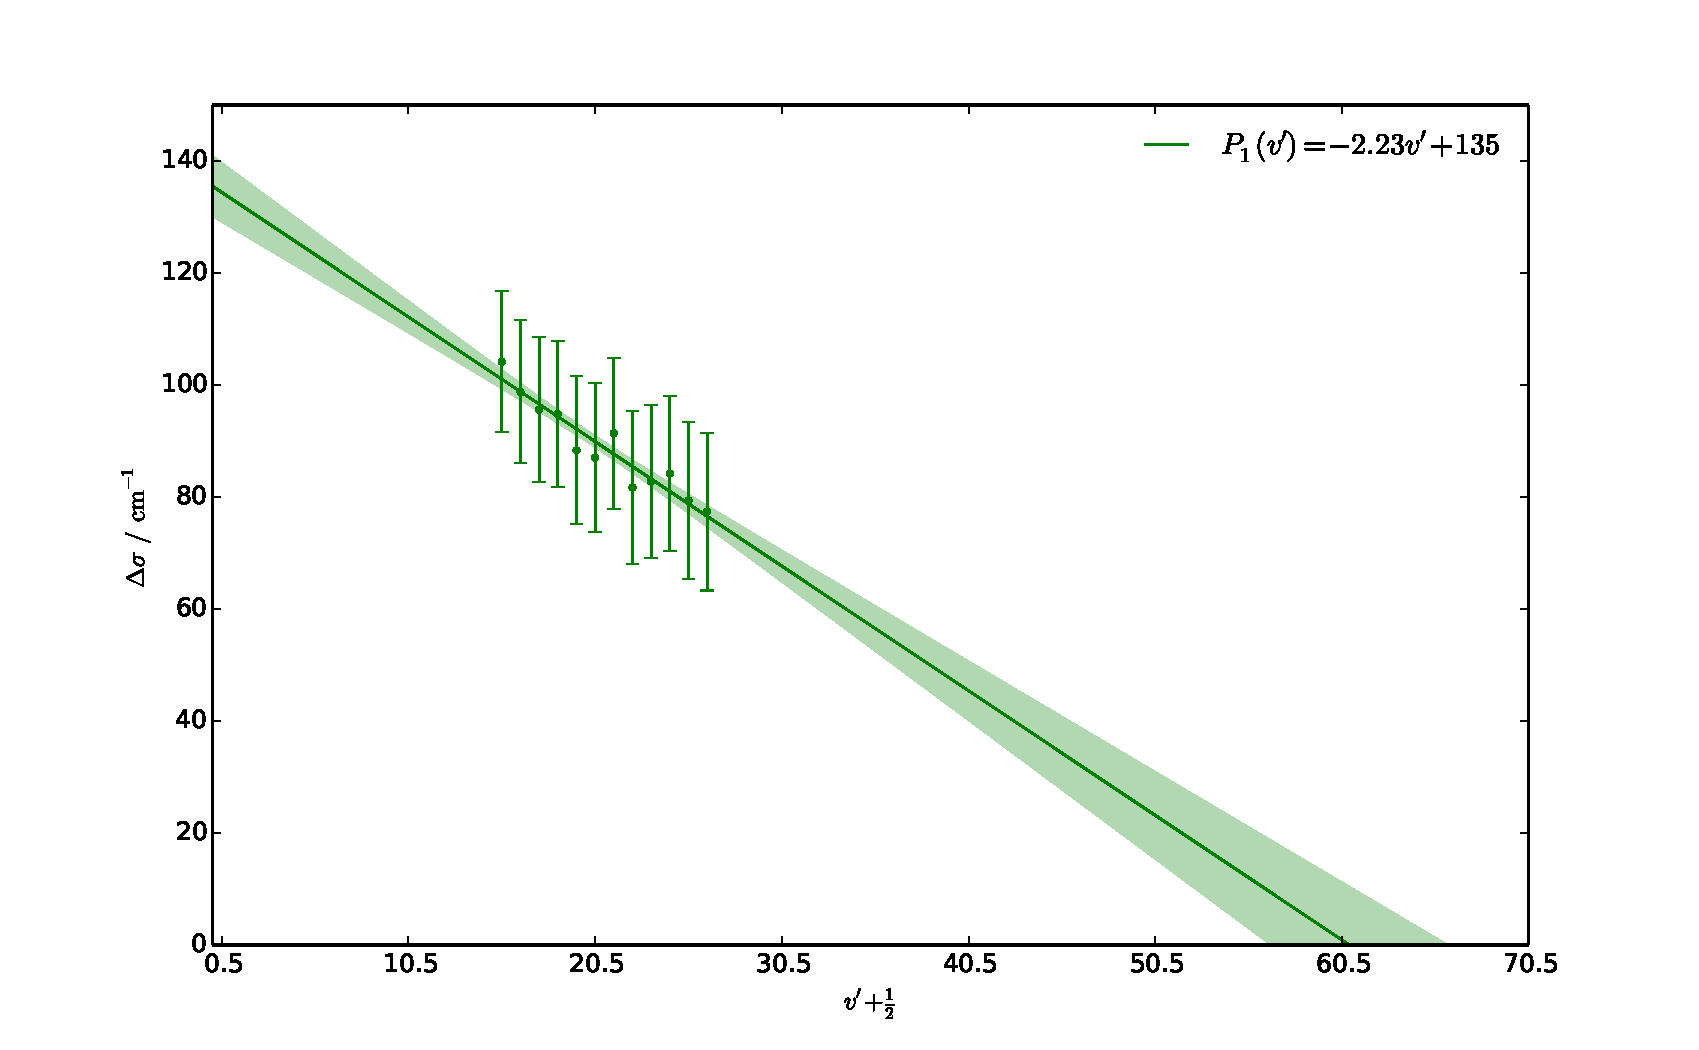
\includegraphics[width=\pltw]{analysis/figures/b_s_1.pdf}
    \caption{Birge-Sponer plot for the progression $v'' = 1 \rightarrow v'$.  
    }
    \label{fig:b_s_1}
\end{figure}

\begin{figure}
    \centering
    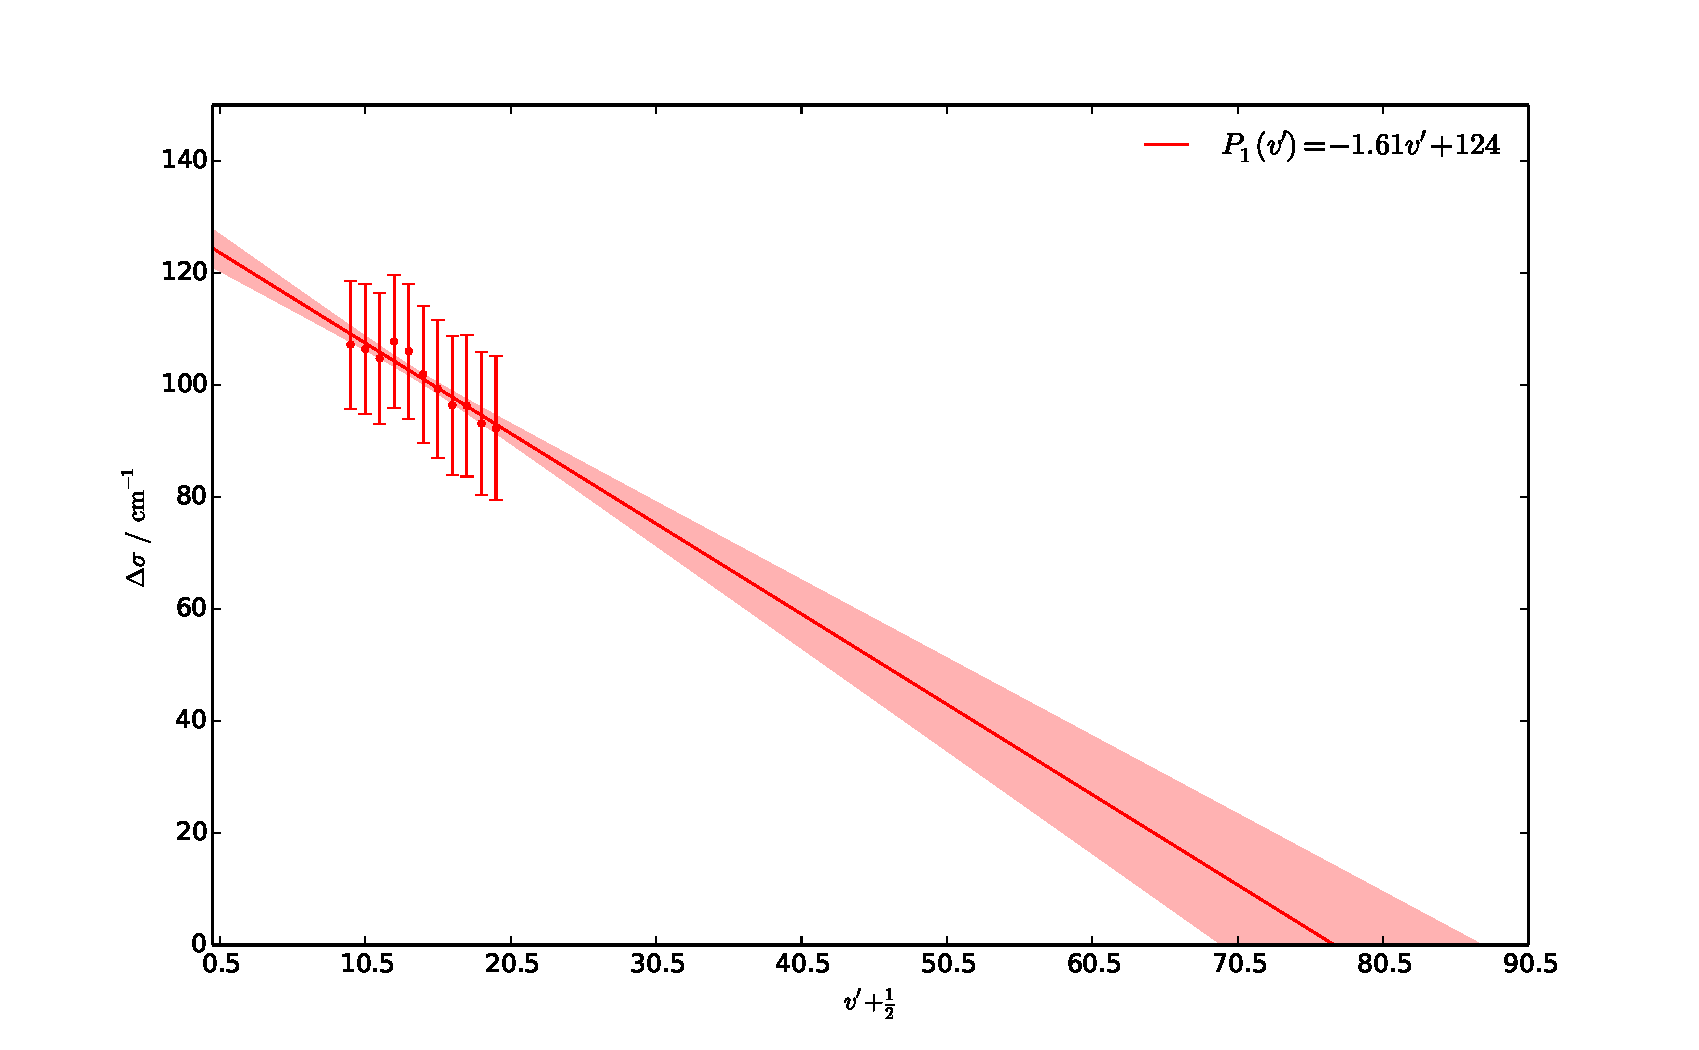
\includegraphics[width=\pltw]{analysis/figures/b_s_2.pdf}
    \caption{Birge-Sponer plot for the progression $v'' = 2 \rightarrow v'$.  
    }
    \label{fig:b_s_2}
\end{figure}

Instead of deducing these variable graphically, we used the expansion 
\eqref{eqn:G(v)_taylor} and did a 
polinomial fit using the linear least square method \cite{cowan1998statistical}. 
As we have only a limited number of points, we used a second degree polynomial
for the zeroth progression and a linear fit for the first and second progression. 
The plots show the best fit as well as estimates for the uncertainties, 
calculated by adding and subtracting the standard deviation of the 
polynome evaluated at each point $v'$. 
In order to maintain readability, we first discuss our results for the zeroth 
progression, and then add the values calculated for the first and second progression 
without further explaining each step, if they are done analogously.

\subsubsection{Progression $v'' = 0 \rightarrow v'$}
The polynomial fit for 
\begin{equation}
    P_2(v') = p_2 {v'}^2 + p_1 v' + p_0
\end{equation}
yields the following values and their uncertainties expressed in form of 
the covariance matrix:
\begin{eqnarray}
    p_2 &=& 2.037\mathrm{e}-03 \cm\\
    p_1 &=& -2.188\mathrm{e}+00 \cm\\
    p_0 &=& 1.337\mathrm{e}+02 \cm\\
    \mathrm{cov}(p_i, p_j) &=& 
    \begin{pmatrix}
        4.027\mathrm{e}-05 &-2.509\mathrm{e}-03 &3.604\mathrm{e}-02 \\
        -2.509\mathrm{e}-03 &1.588\mathrm{e}-01 &-2.317\mathrm{e}+00 \\
        3.604\mathrm{e}-02 &-2.317\mathrm{e}+00 &3.457\mathrm{e}+01 \\
    \end{pmatrix}
\end{eqnarray}
All quantities $p_i$ are given in units of $\cm$, while the entries of the covariance 
matrices are given in $\mathrm{cm^{-2}}$.

Comparing $P_2$ to \eqref{eqn:G(v)_taylor} up to the second order let's us solve for 
the vibrational parameters $w_e$, $w_e x_e$, $w_e y_e$. The system of linear equations in 
${v'}^2, v'$ and $1$ has the solutions:
\begin{eqnarray}
    \omega_e y_e' &=& \frac{p_0}{3} \\
    \omega_e x_e' &=& p_2 - \frac{p_1}{2} \\
    \omega_e'     &=& \frac{11}{12}p_2 - p_1 + p_0.
\end{eqnarray}
Inserting the values from above and doing the error propagation yields 
\begin{eqnarray}
    \omega_e y_e' &=& 6.789\mathrm{e}-04 \cm \nonumber \\
    \omega_e x_e' &=& 1.096\mathrm{e}+00 \cm \nonumber \\
    \omega_e' &=& 1.359\mathrm{e}+02 \cm \nonumber \\
    \mathrm{cov}(p_i, p_j) &=& 
    \begin{pmatrix}
        4.474\mathrm{e}-06 &4.317\mathrm{e}-04 &1.286\mathrm{e}-02 \\
        4.317\mathrm{e}-04 &4.225\mathrm{e}-02 &1.278\mathrm{e}+00 \\
        1.286\mathrm{e}-02 &1.278\mathrm{e}+00 &3.943\mathrm{e}+01 \\
    \end{pmatrix}
\\ \Rightarrow \qquad
    \omega_e y_e' &=& 0.0007 \pm 0.0021 \cm\\
    \omega_e x_e' &=& 1.10 \pm 0.21 \cm\\
    \omega_e' &=& 135.9 \pm 6.3 \cm
\end{eqnarray} 

Using these results, we can calculate the dissociation energies $D_e'$ and $D_0'$. For the 
prior one we get with equation \eqref{eqn:D_e}:
\begin{equation}
    D_e' = \frac{ \omega_e'^2}{ 4  \omega_e x_e'} =\left(4.2 \pm 0.4\right) \times 10^{3} \cm.
\end{equation}
The latter ist calculated using \ref{eqn:D_0}. Before applying this formula, we need to find 
the intersect with the $\Delta \sigma == 0$-axis, which corresponds just to 
$\nu_\mathrm{diss}$. Since we don't observe all transitions, we solve $P_2(v_\mathrm{diss}') = 0$, and 
take the sum over all values $0 < v' + 1/2 < v_\mathrm{diss}'$. In order to estimate the 
uncertainties, we also calculated $v_\mathrm{diss, upper}$ and  $v_\mathrm{diss, lower}$ with 
the corresponding upper und lower limit shown in \ref{fig:b_s_0} and evaluated the sum over 
these polynomes. The dissociation quantum numbers and resulting energies are 
\begin{eqnarray}
    v_\mathrm{diss}' &=& 64.5 \\
    D_0' = \sum_{v' = 0 }^{v'_\mathrm{diss}} P_2 \left (v' + \frac{1}{2} \right ) &=& 4257 \cm \\
    v_\mathrm{diss,\, upper}' &=& 69.5 \\
    D_{0,\, \mathrm{upper}}' &=& 4419 \cm\\
    v_\mathrm{diss,\, lower}' &=& 61.5 \\
    D_{0,\, \mathrm{lower}}' &=& 4122 \cm
\end{eqnarray}
We can summariye these results using the maximum of the distances as the uncertainty of $D_0'$
\begin{equation}
    D_0' = \left(4.26 \pm 0.16\right) \times 10^{3} \cm
\end{equation}

In order to calculate the excitation energy $\sigma_{00}$, we take an arbitrary point of our 
progression and extrapolate the difference between this transition 
$v''= 0 \rightarrow v'$ and the $v'' = 0 \rightarrow v' = 0$ transition. If we take the initial 
point for identifying our progression, $\sigma_{0, 25} = 18319 \pm 10\nm$, in order 
to minimize the error, we get.
\begin{eqnarray}
    \sigma_{00} &:=& G(v' = 0) = G(v' = 25) - (P_2(24.5) - P_2(0.5)) \nonumber \\
                 &\, =& 18364 \pm 12 \cm
\end{eqnarray}
A comparison between the uncertainties of $\sigma_{0, 25}$ and $\sigma_{00}$ shows, 
that the uncertainty of the latter one stems mostly from the given uncertainty 
of $\sigma_{0, 25}$, while the one of the fit is about a magnitude smaller. This, 
as well as simply looking at the plot and recognizing the small deviations from 
the fit indicates, that initial errors might have been assumed to high. 

With the parameters claculated until now, we can deduce the energy $E_\mathrm{diss}$ 
for which the iodine molecule dissociates in the experiment, 
namely the dissociation energy of the $B$-state given in units of the 
energy defined by the ground state. This can be calculated by
\begin{equation}
    E_\mathrm{diss} := \sigma_{00} + D_0'
    \label{eq:E_diss}
\end{equation}
The numerical result for the zeroth progression is
\begin{equation}
    E_\mathrm{diss} = \left(22.62 \pm 0.16\right) \times 10^{3} \cm
\end{equation}


\subsubsection{Progressions $v'' = (1, 2) \rightarrow v'$}
The first an second progression are fitted on a linear function of $v'$, since 
the lack of a higher numerb of points or higher accuray doesn't allow higher order fits.
The function to be fitted is given by
\begin{equation}
    P_1(v') = p_1 v' + p_0.
\end{equation}
In oder to get the vibrational parameters $w_e$ and $w_e x_e$, we compare $P_1$ to 
\eqref{eqn:G(v)_taylor} up to the first order and get the foolowing results: 
\begin{eqnarray}
    w_e x_e' &=& -\frac{p_1}{2} \\
    w_e &=&' p_0 - p_1.
\end{eqnarray}

With these equations, we con now compute the same parameters as done before for the 
zeroth progression:
\begin{itemize}
    \item For $v'' = 1 \rightarrow v'$:
        \begin{eqnarray}
            p_2 &=& -2.225\mathrm{e}+00 \cm \nonumber \\
            p_1 &=& 1.355\mathrm{e}+02 \cm \nonumber \\
            \mathrm{cov}(p_i, p_j) &=& 
            \begin{pmatrix}
                6.430\mathrm{e}-02 &-1.320\mathrm{e}+00 \\
                -1.320\mathrm{e}+00 &2.785\mathrm{e}+01 \\
            \end{pmatrix}
            \\ \Rightarrow \qquad
            \omega_e x_e' &=& 1.113\mathrm{e}+00 \cm \nonumber \\
            \omega_e' &=& 1.378\mathrm{e}+02 \cm \nonumber \\
            \mathrm{cov}(p_i, p_j) &=& 
            \begin{pmatrix}
                1.607\mathrm{e}-02 &6.920\mathrm{e}-01 \\
                6.920\mathrm{e}-01 &3.055\mathrm{e}+01 \\
            \end{pmatrix}
            \\ \Rightarrow \qquad
            \omega_e x_e' &=& 1.11 \pm 0.13 \cm\\
            \omega_e' &=& 137.8 \pm 5.5 \cm \\
            D_e' &=& \left(4.2 \pm 0.4\right) \times 10^{3} \cm \\
            v_\mathrm{diss}' &=& 64.5 \\
            D_0' &=& 4257 \cm \\
            v_\mathrm{diss,\, upper}' &=& 69.5 \\
            D_{0,\, \mathrm{upper}}' &=& 4419 \cm\\
            v_\mathrm{diss,\, lower}' &=& 61.5 \\
            D_{0,\, \mathrm{lower}}' &=& 4122 \cm \\
            \Rightarrow \qquad
            D_0' &=& \left(4.26 \pm 0.16\right) \times 10^{3} \cm
        \end{eqnarray}
        If we pick $v' = 19$ for it being close to $v' = 0$ and the $\Delta G(v' + 1/2)$ 
        for $v' < 19$ close to the linear fit $P_1(v' + 1/2)$, we get the following results for 
        $\sigma_{00}$ and $E_\mathrm{diss}$:
        \begin{eqnarray}
            G'(v' = 19) &=& 17589.9 \pm 9.3 \cm \\
            \sigma_{00} &=& 17605.5 \pm 9.5 \cm \\
            E_\mathrm{diss} &=& \left(21.73 \pm 0.30\right) \times 10^{3} \cm
        \end{eqnarray}
    \end{itemize}
    \begin{itemize}
        \item For $v'' = 2 \rightarrow v'$:
            \begin{eqnarray}
                p_2 &=& -1.613\mathrm{e}+00 \cm \nonumber \\
                p_1 &=& 1.244\mathrm{e}+02 \cm \nonumber \\
                \mathrm{cov}(p_i, p_j) &=& 
                \begin{pmatrix}
                    4.888\mathrm{e}-02 &-6.853\mathrm{e}-01 \\
                    -6.853\mathrm{e}-01 &1.009\mathrm{e}+01 \\
                \end{pmatrix}
                \\ \Rightarrow \qquad
                p_2 &=& -1.61 \pm 0.22 \cm\\
                p_1 &=& 124.4 \pm 3.2 \cm \\
                \omega_e x_e' &=& 8.067\mathrm{e}-01 \cm \nonumber \\
                \omega_e' &=& 1.261\mathrm{e}+02 \cm \nonumber \\
                \mathrm{cov}(p_i, p_j) &=& 
                \begin{pmatrix}
                    1.222\mathrm{e}-02 &3.671\mathrm{e}-01 \\
                3.671\mathrm{e}-01 &1.151\mathrm{e}+01 \\
            \end{pmatrix}
            \\ \Rightarrow \qquad
            \omega_e x_e' &=& 0.81 \pm 0.11 \cm\\
            \omega_e' &=& 126.1 \pm 3.4 \cm \\
            D_e' &=&\left(4.9 \pm 0.4\right) \times 10^{3} \cm \\
            v_\mathrm{diss}' &=& 76.5 \\
            D_0' &=& 4799 \cm \\
            v_\mathrm{diss,\, upper}' &=& 86.5 \\
            D_{0,\, \mathrm{upper}}' &=& 5339 \cm\\
            v_\mathrm{diss,\, lower}' &=& 69.5 \\
            D_{0,\, \mathrm{lower}}' &=& 4383 \cm \\
            D_0' &=& \left(4.8 \pm 0.5\right) \times 10^{3} \cm 
        \end{eqnarray}
        Here we choose $v' = 12$ for the same reasons as before: 
        \begin{eqnarray}
            G'(v' = 12) &=& 16675.1 \pm 8.3 \cm \\
            \sigma_{00} &=& 16686.4 \pm 8.5 \cm \\
            E_\mathrm{diss} &=& \left(21.5 \pm 0.5\right) \times 10^{3} \cm
        \end{eqnarray}
\end{itemize}

\subsubsection{Parameters for the ground state}
With the values for $\Delta G(v' + 1/2)$ calculated in \ref{tab:dG}, we can calculate the vibrational coefficients for 
the ground state by applying equation \eqref{eqn:dG1_2} for $v'' \in \{0, 1, 2\}$:
\begin{eqnarray}
    \Delta G''\left ( \frac{1}{2} \right ) &=& G''(1) - G''(0) \nonumber\\
        &=& (G'(n) - G''(0)) - (G'(n) - G''(1)) \nonumber \\
        &=& \omega_e'' - 2 \omega_e x_e'' \\
    \Delta G''\left ( \frac{3}{2} \right ) &=& G''(2) - G''(1) \nonumber\\
        &=& (G'(n) - G''(1)) - (G'(n) - G''(2)) \nonumber \\
        &=& \omega_e'' - 4 \omega_e x_e'' \\
  \Rightarrow \qquad  \omega_e x_e'' &=& \frac{1}{2} \left ( \Delta G''\left ( \frac{1}{2} \right ) 
        \Delta G''\left ( \frac{3}{2} \right ) \right )
\end{eqnarray}
As seen in table \ref{tab:dG}, we get corresponding pairs for 
$\Delta G''\left ( \frac{1}{2} \right )$ at $v' + 1/2 \in \{18.5, 19.5, \ldots, 26.5\}$ 
and for 
$\Delta G''\left ( \frac{3}{2} \right )$ at $v' + 1/2 \in \{15.5, 16.5, 17.5, 18.5, 19.5\}$.
Taking weighted averages $\overline{\Delta G''\left ( \frac{1}{2} \right )}$ and 
$\overline{\Delta G''\left ( \frac{3}{2} \right )}$, 
where weights are constituited by the reciprocal variances, 
and subtracting yields
\begin{eqnarray}
    \omega_e'' &=& 213.8 \pm 4.6 \cm \\
    \omega_e x_e'' &=& 0.5 \pm 1.4 \cm.
\end{eqnarray}

For small vibrations, we make the approximation of a harmonic oscillator and 
can now calculate classical frequency $f$ and the spring constant $k$ with 
\eqref{eqn:freq}:
\begin{eqnarray}
    f_e'' &=& \left(1.282 \pm 0.028\right) \times 10^{12} \mathrm{Hz} \\
    k_e'' &=& 6.84 \pm 0.30 \mathrm{\frac{kg}{s^2}}
\end{eqnarray}

Approximating the ground state for low vibrational modes with the morse function, 
we can calculate the dissociation energy of the ground state with the values for 
$\omega_e''$ and $\omega_e x_e''$ with \eqref{eqn:D_e}:
\begin{equation}
    D_e'' =\left(25 \pm 74\right) \times 10^{3} \cm
\end{equation}
We can compare this value with a second one, which we get from approximating the 
dissociation energy as the difference between $E_\mathrm{diss}$ and the difference in 
energy of the two resulting dissociated atoms. If dissociation takes place directly 
from the ground level, the resulting atoms are both in their ground states $^2 P_{3/2}$, 
while for dissociation from the excited state, one of the atoms is found in the first 
excited state $2^ P_{1/2}$. The energy difference between the two states is given by 
$\Delta E = 7603.15 \cm$~\cite{nist}. We thus get the following results for the energy 
levels calculated with each of the three progressions:
\begin{eqnarray}
    D_{e, i}'' &:=& E_\mathrm{diss,\, i} - \Delta E\\
    D_{e, 0}'' &\ =&\left(15.02 \pm 0.16\right) \times 10^{3} \cm \\
    D_{e, 1}'' &\ =&\left(14.13 \pm 0.30\right) \times 10^{3} \cm \\
    D_{e, 2}'' &\ =&\left(13.9 \pm 0.5\right) \times 10^{3} \cm
\end{eqnarray}
In the literature, this value is given as $12452.5 \pm 1.5 \cm$ \cite{leroy1970spectroscopic}. 
The fact, that this value 
does not coicinde with our measured value can be due to several factors. 
First of all, take as little points as we did, the fits for the progressions 
naturally don't return very accurate results. Secondly, the Birge-Sponer extrapolation 
induces further errors. Third, the theoretical assumptions are only valid to a certain order. 
It is, however,  not within the scope of this report to assess the validity or precision of 
the assumptions made theoretically.

\subsubsection{Morse potential}
We can use the derived parameters to calculate and plot the Morse potential for the 
excited state. For that, we calculate $a'$ with equation \eqref{eqn:wx_e} and 
use the $r_e' = 3.035 \AA$ calculated before \eqref{eqn:r_e1}:
\begin{eqnarray}
    a_i &=& \sqrt{\frac{4 \pi c \mu {\omega_e x_e}_i}{\hbar}} \\
    a_0' &=& 2.02 \pm 0.19 \AA^{-1} \\
    a_1' &=& 2.04 \pm 0.12 \AA^{-1} \\
    a_2' &=& 1.74 \pm 0.12 \AA^{-1} \\
\end{eqnarray}
For the value $a_0'$ obtained from the zeroth progression, we plot the Morse potential 
in figure \ref{fig:morse}.

\begin{figure}
    \centering
    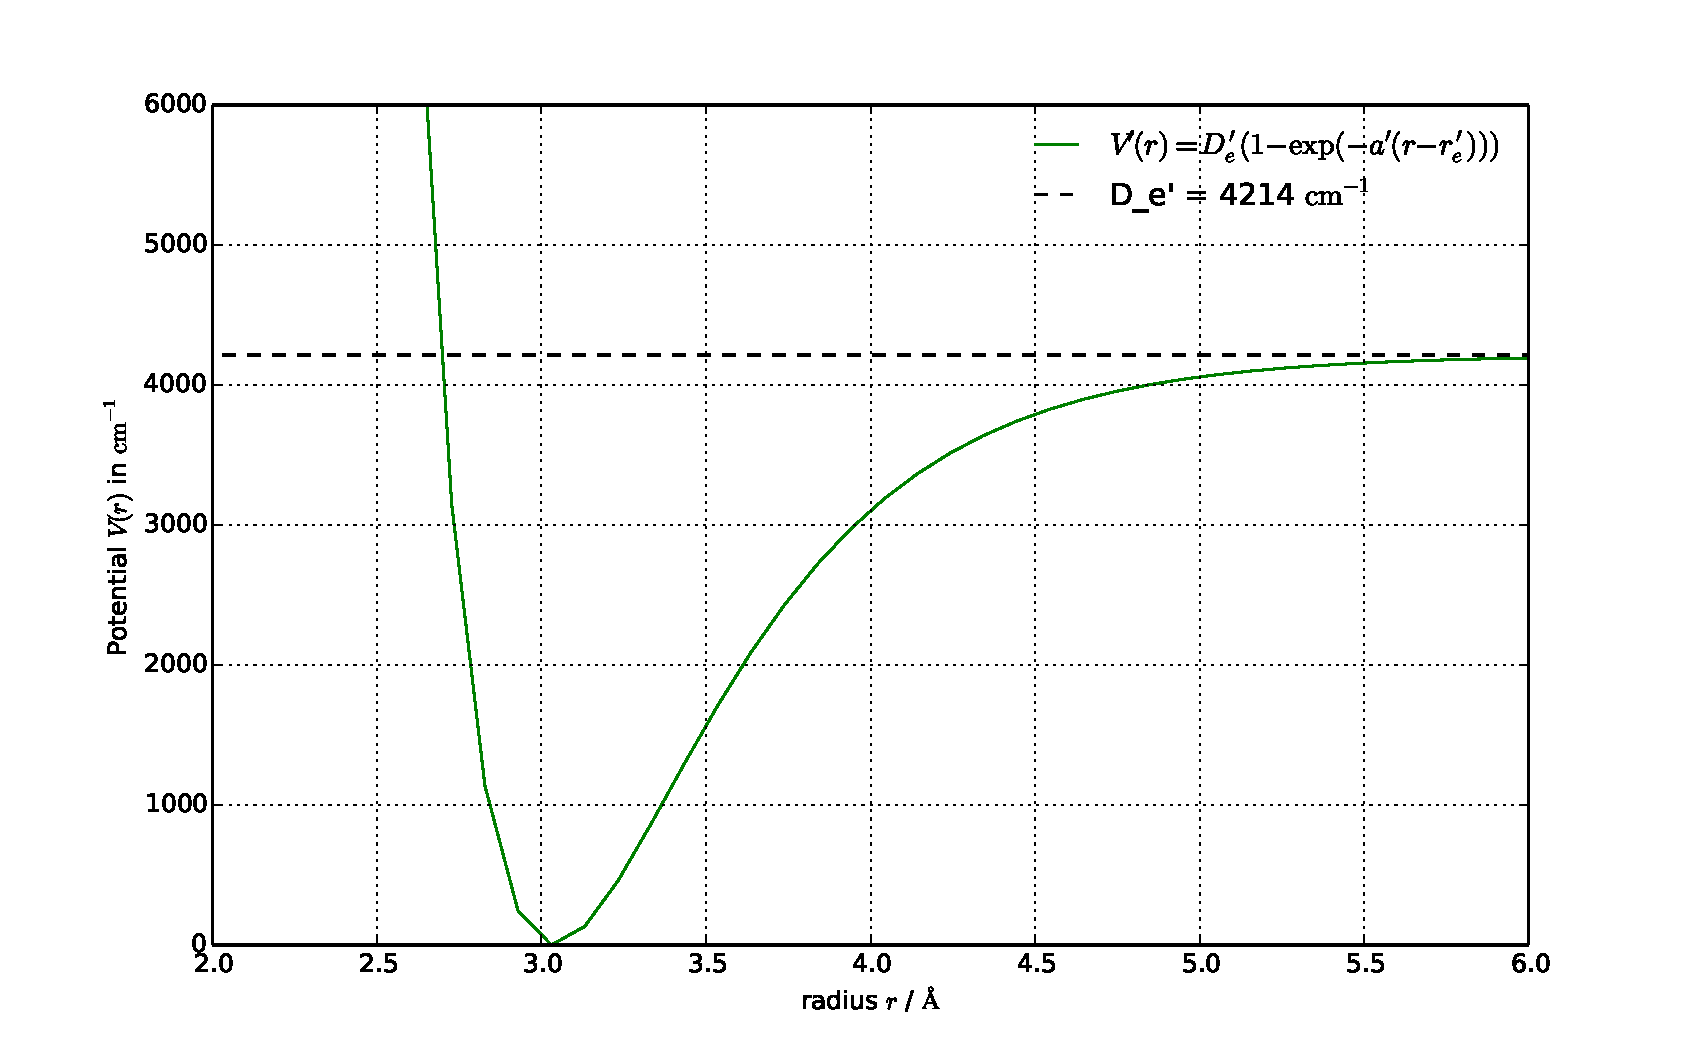
\includegraphics[width=\pltw]{analysis/figures/morse_plot_0.pdf}
    \caption{Morse plot for the first excited state 
    $B ^3\Pi_{\sigma \, \mathrm{u}}^{+}$ of the iodine 2 molecule. 
    The parameters $a' = 2.02 \pm 0.19\ \AA^{-1}$ and dissociation energy 
    $D_e' = \left(4.2 \pm 0.4\right) \times 10^{3} \cm$
    are obtained from the progression $v'' = 0 \rightarrow v'$. 
    The radius $r_e' = 3.035 \AA$ is calculated from literature values in \eqref{eqn:r_e1}. 
    }
    \label{fig:morse}
\end{figure}














\begin{comment}

We immediately see, that the parameter $\omega_e y_e'$ is practically zero within its 
bound of uncertainty - the number of points is not enough to calculate this parameter 
up to a desirable accuracy. 


The literature values are given by:
\begin{eqnarray}
    {\omega_e'}_\mathrm{\ lit} &=& 125.69 \cm \cite{nist} \\
    {\omega_e x_e'}_\mathrm{\ lit} &=& 0.764 \cm \cite{nist} \\
    {\omega_e y_e'}_\mathrm{\ lit} &=& -0.00567 \cm \cite{steinfeld1965spectroscopic}
\end{eqnarray} 
\end{comment}


